\documentclass[onecolumn, 12pt]{IEEEtran}

\usepackage{amsfonts,amsmath,amssymb,amsthm}
\usepackage{graphicx}

\begin{document}

\title{Template for Report}
\author{Author 1, Author 2}

\maketitle

\section{Introduction}
In this section, a general description of the problem under consideration is provided. 
As soon as the reader completes the introduction, (s)he should be aware of what will 
be discussed in the main body and the possible contributions, e.g. how the problem was 
solved. It is suggested to briefly describe, in words, the structure of the report and 
how it is organized. The report could be single or double column.

\section{Problem Formulation and Solution}
This section contains the analytical presentation of the problem and the solution steps. 
It could be organized in many different subsections, depending on the structure of the 
problem itself (one problem or small tasks) and the personal choice of presentation.

\subsection{Part 1}
The first part of the problem along with its solution goes here. It is suggested to number 
any equations that will be referenced later in text.
\begin{equation} \label{eq:Eq1}
y(n)=x(n)+z(n)
\end{equation}
The above equation is referred to as \eqref{eq:Eq1}, anywhere the text. 

\subsection{Part 2}
The report continues with the second part, and so on until the whole problem has been 
addressed and solved. If someone wants to refer, at some point, to external material 
then proper citation and referencing is needed, e.g. the coursebook in signal theory 
\cite{HanOttHjalm}. Figures and images are placed at the top/bottom of the page to 
avoid interrupting the text flow.

\begin{figure}[b]
\begin{center}
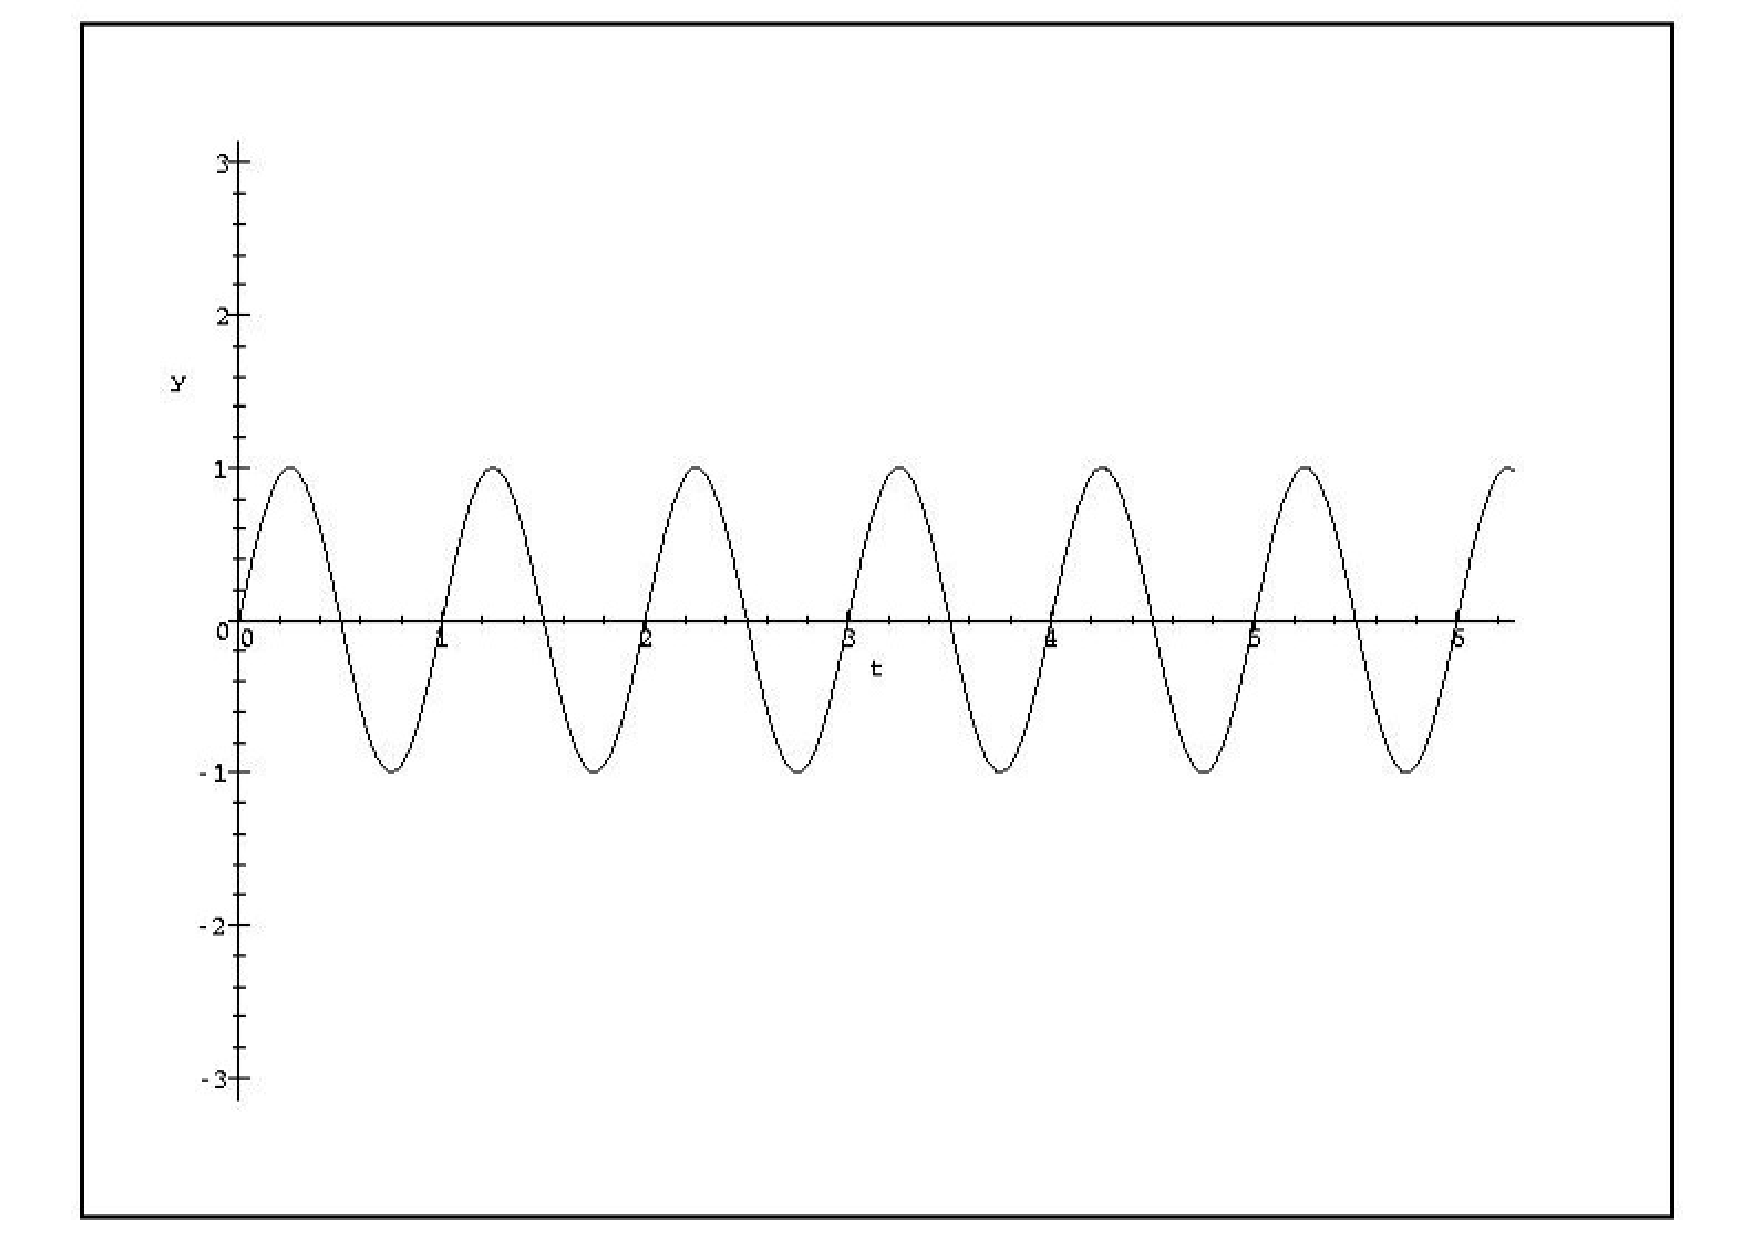
\includegraphics[trim=1.8cm 5.1cm 2.8cm 4.9cm, clip=true, totalheight=0.2\textheight,width=0.45\textwidth]{Sinusoid.pdf}
\end{center}
\vspace{-0.4cm}
\caption {Sample figure.}
\label{fig:Fig1}
\end{figure}

\section{Conclusions}
A summary of the findings is provided here. It is also good to highlight the most important 
parts of the solution and briefly discuss some implications, e.g. in real-world applications,
or extensions deserving further investigation.

\begin{thebibliography}{1}

\bibitem{HanOttHjalm}
P. Handel, R. Ottoson, H. Hjalmarsson, \emph{Signal Theory}, KTH, 2012

\end{thebibliography}

\end{document}
